\documentclass[tikz,border=5pt]{standalone}
\usepackage[utf8]{inputenc}
\usepackage[T1]{fontenc}
\usepackage{lmodern,amsmath,amssymb}
\usepackage[american]{circuitikz}
\usepackage{pgfplots}
\pgfplotsset{compat=1.18}
\usetikzlibrary{circuits.logic.US,positioning,calc,arrows.meta,patterns,shapes.geometric}
\definecolor{Primary}{HTML}{1F77B4}
\begin{document}
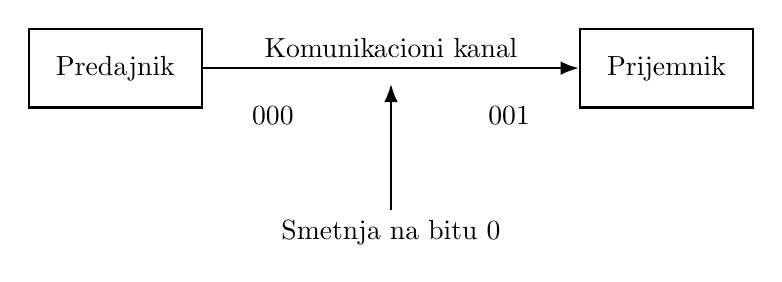
\begin{tikzpicture}[>=Latex,thick]
\node[draw,minimum width=2.2cm,minimum height=1cm](tx)at(0,0){Predajnik};\node[draw,minimum width=2.2cm,minimum height=1cm](rx)at(7,0){Prijemnik};
\draw[->](tx)--(rx)node[midway,above]{Komunikacioni kanal};\node at(2,-.6){000};\node at(5,-.6){001};\draw[->](3.5,-1.8)node[below]{Smetnja na bitu 0}--(3.5,-.2);
\end{tikzpicture}
\end{document}
